  \pagebreak
  \section{Actividad Práctica}
    Se propone realizar las mediciones de \textbf{potencias} y \textbf{factor de potencia}, y posteriormente,
    la \textbf{corrección} de dicho factor, en una carga reactiva, la cual se trata de un tubo fluorescente 
    común. Este mismo se encuentra preparado junto a un circuito de medición que provee la cátedra. En la 
    Figura~\ref{fig:CircuitoMedicion} se puede apreciar un esquema del mismo y una foto real.

    \begin{figure}[H]
      \centering
        \begin{subfigure}[t]{0.7\textwidth}
          \centering
          \frame{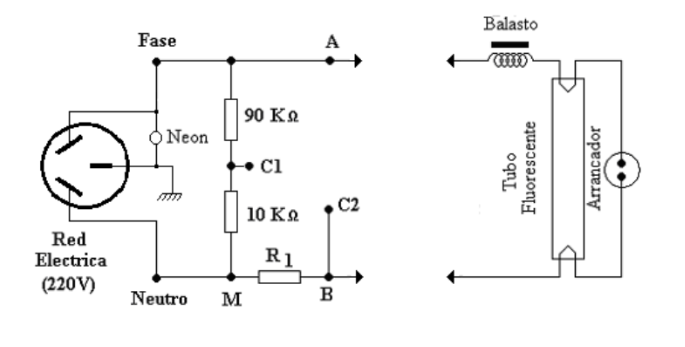
\includegraphics[width=\textwidth]{Imagenes/ActividadPractica/EsquemaCircuito.png}}
          \caption{Esquema.}
          \label{fig:EsquemaCircuito}
        \end{subfigure}
        \begin{subfigure}[t]{0.7\textwidth}
          \centering
          \frame{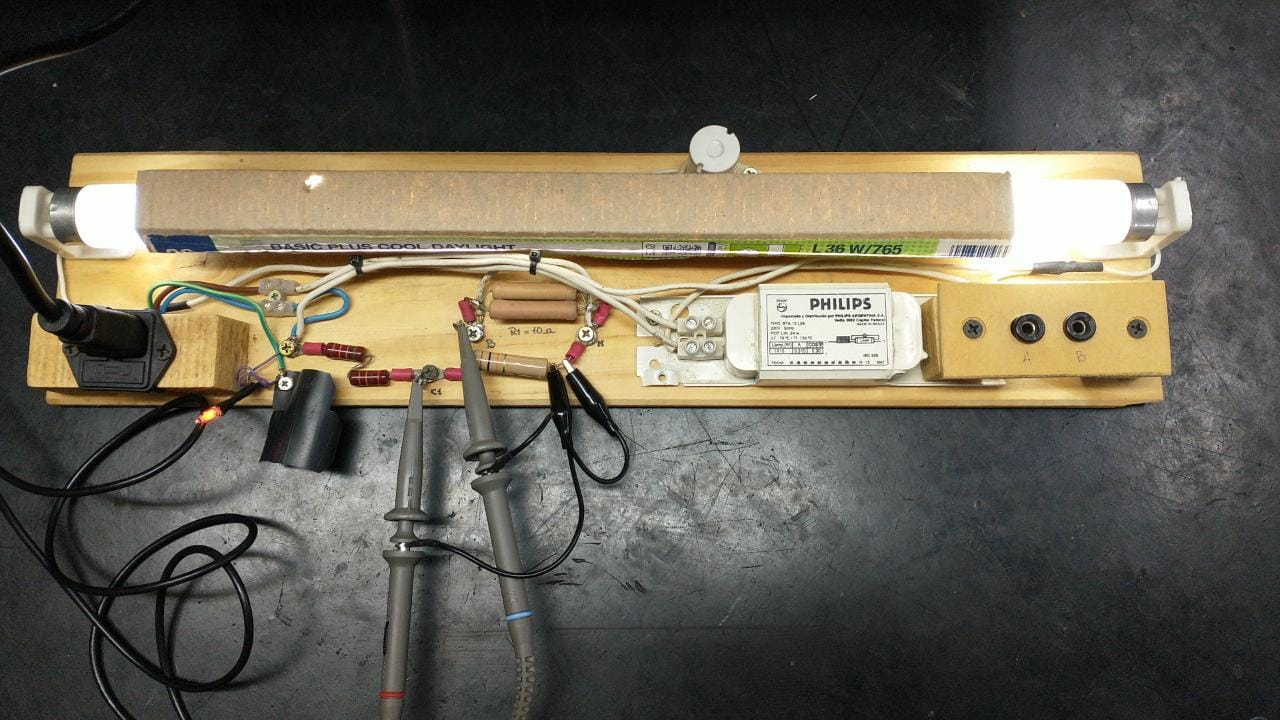
\includegraphics[width=\textwidth]{Imagenes/ActividadPractica/FotoRealCircuito.jpeg}}
          \caption{Foto real.}
          \label{fig:FotoRealCircuito}
        \end{subfigure}
      \caption{Circuito de medición propuesto por la cátedra.}
      \label{fig:CircuitoMedicion}
    \end{figure}

    En el circuito de medición se puede apreciar el punto \textbf{M}, en el cual se conecta la tierra del osciloscopio
    por medio de sus puntas. Por esta razón, es importante y obligatorio el uso de un \textbf{transformador de aislación},
    el cual tiene una de relación 1:1, y tiene como función crear una barrera física de aislación
    entre los equipos/circuitos con los cuales se trabaja y la red. Esto se justifica con que, la diferencia de
    potencial entre \textit{neutro} y \textit{tierra} de la red no es cero (idealmente debería serlo), para este caso, dicho
    valor es de aproximadamente $\mathbf{1,27\ V}$. Este valor generaría un flujo de corriente a través del osciloscopio 
    directo a la \textit{tierra}, lo cual podría dañar el instrumento, y además, provocaría que el diferencial se active.

    Siguiendo con el análisis del circuito de medición, se puede apreciar un divisor resistivo. Esto permite que, en el
    punto \textbf{C1} se pueda medir la \textbf{décima parte} de la tensión de entrada. Luego, en el punto \textbf{C2} 
    se mide la corriente de entrada por Ley de Ohm, ya que el valor de la resistencia es $\mathbf{R_1=10\ \Omega}$.
    
    Se aclara que el kit utilizado no respeta el código de colores de los cables, siendo la fase y el neutro de color azul
    y marrón respectivamente.

      \subsection{Medición de potencia activa y factor de potencia} 
    Las conexiones explicadas se representan en el esquema de la Figura~\ref{fig:EsquemaConexiones}.
    Se hace uso de las atenuaciones que ofrece el osciloscopio digital, de forma tal que los valores
    que se miden sean exactamente los valores reales. Es decir, para el \textbf{canal 1}, en cual se mide
    la \textit{tensión de entrada} $\mathbf{V_i}$, se coloca una \textbf{atenuación x100} (x10 de la punta
    y x10 del divisor resistivo), y para el \textbf{canal 2}, en el cual se mide la \textit{corriente de entrada}
    $\mathbf{I_i}$ de forma indirecta por Ley de Ohm, se coloca una atenuación \textbf{atenuación x1}
    (debido a que $R\textsubscript{1}=10\ \Omega$).

    \begin{figure}[H]
      \centering
      \frame{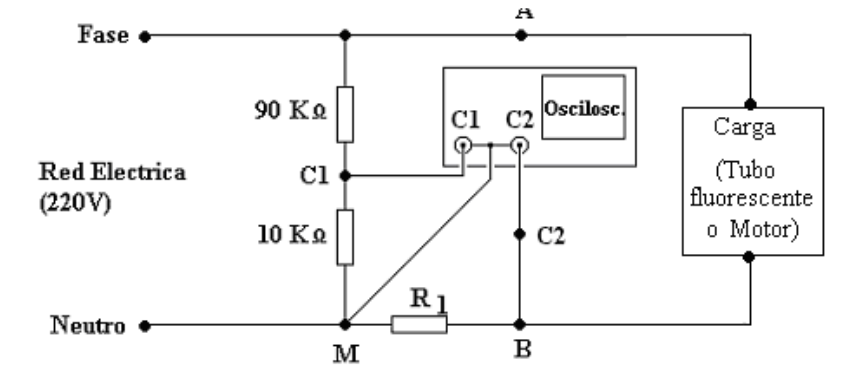
\includegraphics[width=0.7\textwidth]{Imagenes/ActividadPractica/EsquemaConexiones.png}}
      \caption{Esquema de conexiones para las mediciones.}
      \label{fig:EsquemaConexiones}
    \end{figure}

    \subsubsection{Medición de los módulos de tensión y corriente de entrada}
      En la Figura~\ref{fig:Vi_Ii} se puede ver los valores obtenidos al realizar la medición, los cuales
      se obtienen como valores \textit{root main square} (RMS), ya que se utilizan para el cálculo de 
      potencias. Las mediciones son:
      
      \begin{equation*}
        \boxed{V_{i_{RMS}} =  213 \ [V]} \hspace{20pt} ; \hspace{20pt} \boxed{I_{i_{RMS}} = 333\ [mA]}\ .
      \end{equation*}
      
      \begin{figure}[H]
        \centering
        \frame{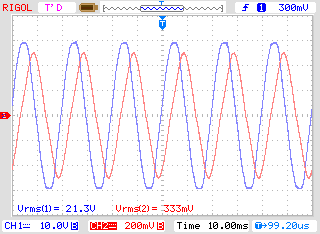
\includegraphics[width=0.4\textwidth]{Imagenes/ActividadPractica/MedicionDePotenciasYFdP/Exp1_1_Vin-Iin.png}}
        \caption{Medición de tensión y corriente de entrada con el osciloscopio.}
        \label{fig:Vi_Ii}
      \end{figure}
  
    \subsubsection{Medición de la diferencia de fase de la tensión y corriente de entrada}
    A continuación, se procede a calcular la \textbf{diferencia de fase} de la tensión y corriente de entrada.
    En la Figura~\ref{fig:DiferenciaDeFase} se aprecia la medición con el osciloscopio en modo dual y en modo X-Y.

    \begin{figure}[H]
      \centering
      \begin{subfigure}[h]{0.4\textwidth}
        \centering
        \frame{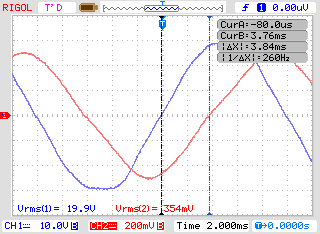
\includegraphics[width=\textwidth]{Imagenes/ActividadPractica/MedicionDePotenciasYFdP/Exp1_2_DiferenciaDeFaseEnSegundos.png}}
        \caption{Medición en modo dual.}
        \label{fig:DiferenciaDeFaseEnSegundos}
      \end{subfigure}
      \hspace{20pt} 
      \begin{subfigure}[h]{0.4\textwidth}
        \centering
        \frame{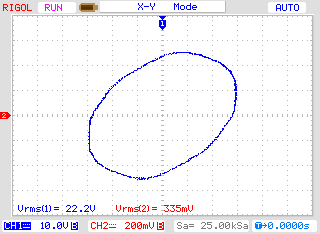
\includegraphics[width=\textwidth]{Imagenes/ActividadPractica/MedicionDePotenciasYFdP/Exp1_4_FiguraDeLissajous.png}}
        \caption{Medición en modo X-Y.}
        \label{fig:FiguraLissajous}
      \end{subfigure}
      \caption{Medición de diferencia de fase.}
      \label{fig:DiferenciaDeFase}
    \end{figure}

    \subsubsection*{Método 1: medición en modo dual}
    Simplemente, se procede a realizar una regla de tres simple, basándose en la Figura~\ref{fig:DesfaseEnSegundos}, mediante el
    semiperíodo de la tensión de entrada y la diferencia en segundos entre las señales. Por lo tanto, la diferencia de
    fase es

    \begin{align*}
      9,92\ ms &\longrightarrow 180\ ^{\circ} (semiperiodo) \\
      3,82\ ms &\longrightarrow \varphi = \dfrac{3,84\ ms \cdot 180\ ^{\circ}}{9,92\ ms} \hspace{20pt} \Longrightarrow \hspace{20pt} \Aboxed{\varphi=69,67\ ^{\circ}}\ .
    \end{align*}

    \begin{figure}[H]
      \centering
      \begin{subfigure}[h]{0.4\textwidth}
        \centering
        \frame{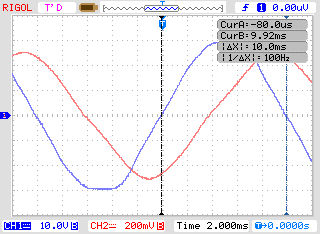
\includegraphics[width=\textwidth]{Imagenes/ActividadPractica/MedicionDePotenciasYFdP/Exp1_9_SemiperiodoEnSegundos.png}}
        \caption{Semiperíodo en segundos.}
        \label{fig:SemiperiodoEnSegundos}
      \end{subfigure}
      \hspace{20pt} 
      \begin{subfigure}[h]{0.4\textwidth}
        \centering
        \frame{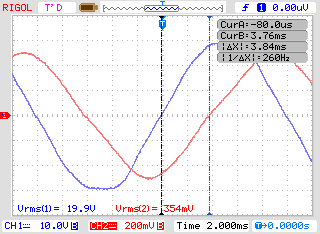
\includegraphics[width=\textwidth]{Imagenes/ActividadPractica/MedicionDePotenciasYFdP/Exp1_2_DiferenciaDeFaseEnSegundos.png}}
        \caption{Desfase de las señales en seg.}
        \label{fig:DiferenciaDetiempoDeLasSeñales}
      \end{subfigure}
      \caption{Medición de diferencia de fase en modo dual.}
      \label{fig:DesfaseEnSegundos}
    \end{figure}

    \subsubsection*{Método 2: medición en modo X-Y}
    Este método se basa en el uso de la figura de Lissajous mostrada en el osciloscopio. Las mediciones se pueden ver en la 
    Figura~\ref{fig:DesfaseConLissajous}. En base a la ecuación~(\ref{eqn:AngDeDesf}) se calcula el valor de la 
    \textbf{diferencia de fase}
    
    \begin{align*}
      \varphi = sen ^{-1} \left( \dfrac{A}{B} \right) = sen ^{-1} \left( \dfrac{0,944\ V}{1,01\ V} \right) \hspace{20pt} \Longrightarrow \hspace{20pt} \Aboxed{\varphi = 69,17\ ^{\circ}}\ .
    \end{align*}

    \begin{figure}[H]
      \centering
      \begin{subfigure}[h]{0.4\textwidth}
        \centering
        \frame{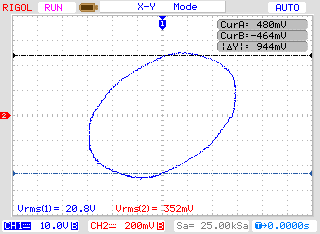
\includegraphics[width=\textwidth]{Imagenes/ActividadPractica/MedicionDePotenciasYFdP/Exp1_6_CortesEjeYFigLis.png}}
        \caption{Valores de corte de la figura en el eje vertical (A).}
        \label{fig:CortesEjeVertical_Lissajous}
      \end{subfigure}
      \hspace{20pt} 
      \begin{subfigure}[h]{0.4\textwidth}
        \centering
        \frame{\includegraphics[width=\textwidth]{Imagenes/ActividadPractica/MedicionDePotenciasYFdP/Exp1_7_MáximosEjeVertical.png}}
        \caption{Valores máximos de la figura en el eje vertical (B).}
        \label{fig:MaximosEjeVertical_Lissajous}
      \end{subfigure}
      \caption{Medición de diferencia de fase en  modo X-Y.}
      \label{fig:DesfaseConLissajous}
    \end{figure}


    Con las mediciones anteriores ya realizadas, se calculan las potencias \textbf{activa} (P), \textbf{reactiva} (Q)
    y \textbf{aparente} (S), con el uso de las ecuaciones~(\ref{eqn:PotActTot}), (\ref{eqn:PotReacTot}) y 
    (\ref{eqn:PotApaTot}) respectivamente

    \begin{align*}
      P &= V_i  I_i  \cos(\varphi) = 213\ V \cdot 0,333\ A \cdot \cos(69,17\ ^{\circ}) 
                                \hspace{20pt} \therefore \hspace{20pt} \Aboxed{P = 25,22\ [W]} \\
      Q &= V_i  I_i  \sen(\varphi) = 213\ V \cdot 0,333\ A \cdot \sin(69,17\ ^{\circ}) 
                                \hspace{20pt} \therefore \hspace{20pt} \Aboxed{Q = 66,29\ [VAR]} \\
      S &= \sqrt{P^2 + Q^2} =  \sqrt{(25,22\ W)^2 + (66,29\ VAR)^2}
                                \hspace{20pt} \therefore \hspace{20pt} \Aboxed{S = 70,92\ [VA]} \ .
    \end{align*}

    \noindent De la misma forma, con la ecuación~(\ref{eqn:fpFinal}) se calcula el factor de potencia \textbf{fp}
    \begin{align*}
      fp = cos(\varphi) = cos(69,17 ^{\circ}) \hspace{20pt} \therefore \hspace{20pt} \Aboxed{fp = 0,36}\ .
    \end{align*}




      \subsection{Correción del factor de potencia}
    \subsubsection{Cálculo del capacitor de compensación}
      
       Usando la ecuación~(\ref{eqn:CorrecFp}) se determina el valor del capacitor de compensación

      \begin{align*}
        %\varphi = sen ^{-1} \left( \dfrac{A}{B} \right) = sen ^{-1} \left( \dfrac{0,944\ V}{1,01\ V} \right) \hspace{20pt} \Longrightarrow \hspace{20pt} \Aboxed{\varphi = 69,17\ ^{\circ}}\ .
        C = \frac{25,22 [W] \cdot tg(69,67 ^{\circ} )}{(213[V])^2 \cdot 2 \cdot \pi \cdot 50[Hz] }  \hspace{20pt} \Longrightarrow \hspace{20pt} \Aboxed{C = 4,776 [ \mu F]}.
      \end{align*}

        También es posible encontrar el valor del capacitor conociendo el factor de potencia, de acuerdo
        con el gráfico siguiente:

        \begin{figure}[H]
          \centering
            \frame{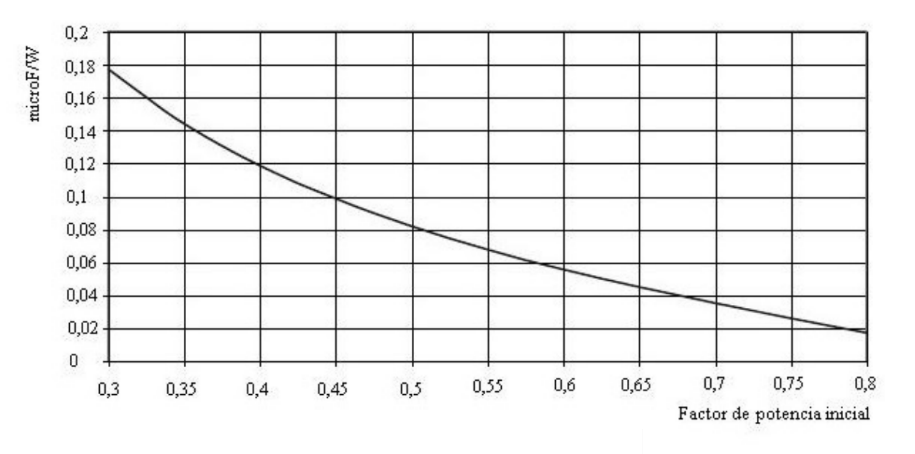
\includegraphics[width=0.7\textwidth]{Imagenes/ActividadPractica/CorreccionDeFdP/Curva Capa_FDP.png}}
            \caption{Curva Capacitancia-Factor de Potencia.}
            \label{fig: Curva Cap_FDP}
        \end{figure}

        Que corresponde con un valor de Capacitancia de 3,63 [$\mu$F], 

    \subsubsection{Medicion del factor de potencia corregido}

          Como se dificulta medir la diferencia de fase entre una señal y otra con el método del modo X-Y,
          se procede a determinar dicho desfasaje a partir de las señales en el dominio del tiempo. 
          Se dispone de un capacitor de valor 4,7[$\mu$F], con lo cual se cumple el requisito presentado
          anteriormente. Se procede a la conexión del mismo, y se observa en el osciloscopio el resultado.
        
        \begin{figure}[H]
          \centering
          \frame{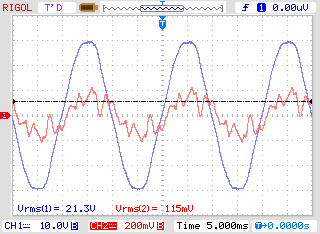
\includegraphics[width=0.7\textwidth]{Imagenes/ActividadPractica/CorreccionDeFdP/Exp2_11_Vin-Iin-ConCapacitor.png}}
          \caption{Señal resultante al agregar un capacitor.}
          \label{fig: Señal_Correccion}
        \end{figure}

        Se observa una importante cantidad de armónicos sumados a la señal de corriente, ésto debido
        a la deformación provocada por la carga conectada a la red.

         Con los nuevos valores de tension y corriente, se determina el valor de la nueva potencia 
         aparente

        \begin{align*}
          S = V_{rms}I_{rms}  \hspace{20pt} S=213\ [V]*0,115\ [A] \Longrightarrow \hspace{20pt} \Aboxed{S = 4,776 [VA]}.
        \end{align*}

          Adicionalmente, puede determinarse el factor de potencia corregido, a partir de las señales
          obtenidas en el tiempo. El principal problema es la cantidad de armónicos montados sobre 
          la señal de corriente, para resolverlo se debe aplicar un filtro pasa bajos a la misma, de
         ésta manera, es más sencillo realizar los cálculos.

        \begin{figure}[H]
          \centering
          \frame{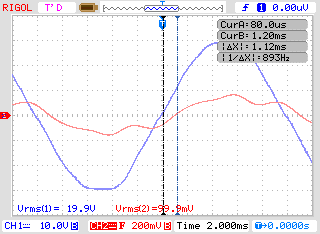
\includegraphics[width=0.7\textwidth]{Imagenes/ActividadPractica/CorreccionDeFdP/Exp2_15_Vin-Iin-ConCapacitorYFiltroEnOsc.png}}
          \caption{Medición del desfasaje de tensión y corriente.}
          \label{fig: Desfasaje tensión-corriente.}
        \end{figure}  

        Se tiene un semiperiódo de 10[ms] (lo que se corresponde con la frecuencia de la red de 50Hz),
        que equivalen a una pulsación de 180° , y usando la relación de tiempo/división del 
        osciloscopio junto con la relación entre ángulo y tiempo , se determina la correspondencia 
        en grados del desfasaje de la señal

        \begin{align*}
          \varphi = sen ^{-1} \left( \dfrac{t_{0}[ms] \cdot 180\ ^{\circ}}{0,5 \cdot T[ms]} \right) = sen ^{-1} \left( \dfrac{1,12[ms] \cdot 180\ ^{\circ}}{10[ms]} \right) \hspace{20pt} \Longrightarrow \hspace{20pt} \Aboxed{\varphi = 20,16\ ^{\circ}}\ .
        \end{align*}    

   

